\begin{frame}{The (under)sampling case}{Where will we see the molecule?}

\underline{Recorded position:} $Y$ is the position of the laser when the molecule is detected;

\[\mathds{P}(Y = y_{r}) = (\mathcal{I}_{\mathds{P}}(t_{0}, \cdot) \star f_{x})(y_{r})\]

\begin{figure}[H]
	\label{mapping1}\caption{The sampling design}
	\centering
    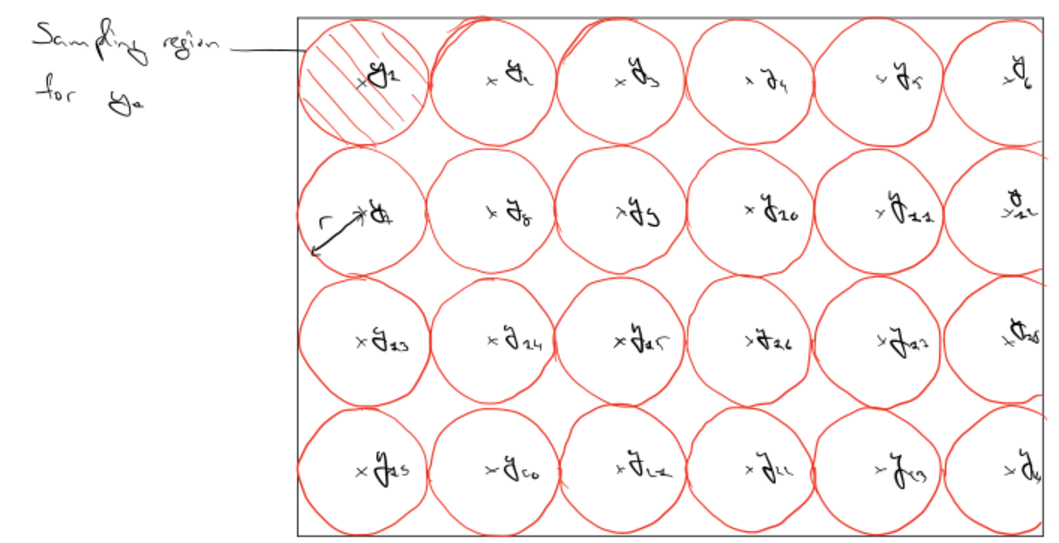
\includegraphics[scale = .4, keepaspectratio]{modelling/sampling/undersampling.pdf}
\end{figure}
\end{frame}